\exercisesection

\begin{exercise} \label{exercise 2.4.1}
Label the following statements as true or false.
In each part, \(V\) and \(W\) are vector spaces with ordered (finite) bases \(\alpha\) and \(\beta\), respectively, \(\T: V \to W\) is linear, and \(A\) and \(B\) are matrices.
\begin{enumerate}
\item \(([\T]_{\alpha}^{\beta})^{-1} = [\T^{-1}]_{\alpha}^{\beta}\).
\item \(\T\) is invertible if and only if \(\T\) is one-to-one and onto.
\item \(\T = \LMTRAN_A\), where \(A = [\T]_{\alpha}^{\beta}\).
\item \(M_{2 \X 3}(F)\) is isomorphic to \(F^5\).
\item \(\POLYNF\) is isomorphic to \(\mathcal{P}_m(F)\) if and only if \(n = m\).
\item \(AB = I\) implies that \(A\) and \(B\) are invertible.
\item If \(A\) is invertible, then \((A^{-1})^{-1} = A\).
\item \(A\) is invertible if and only if \(\LMTRAN_A\) is invertible.
\item \(A\) must be square in order to possess an inverse.
\end{enumerate}
\end{exercise}

\begin{proof} \ 

\begin{enumerate}
\item False.
    First, \(\T\) should be invertible to make \(\T^{-1}\) and \(([\T]_{\alpha}^{\beta})^{-1}\) well defined.
    Second, if \(\T\) is invertible, then by \THM{2.18}, \(([\T]_{\alpha}^{\beta})^{-1} = [\T^{-1}]_{\beta}^{\alpha}\).
\item True, this is just true for normal functions.
\item False. the domain and codomain of \(\T\) and \(\LMTRAN_A\) are not necessarily the same.
\item False, \(\dim(M_{2 \X 3}(F)) = 6 \ne 5 = \dim(F^5)\), so by \THM{2.19}, they are not isomorphic to each other.
\item True, \(\POLYNF\) is isomorphic to \(\mathcal{P}_m(F)\), if and only if (by \THM{2.19}) their dimension are equal, that is, if and only if \(n = m\).
\item False, by \DEF{2.13} we also need to check \(BA = I\); and \(A, B\) \emph{must be squares of the same size}.
    Counter example:
    \[
        \left(\begin{array}{lll}
            1 & 0 & 0 \\
            0 & 1 & 0
        \end{array}\right)
        \left(\begin{array}{ll}
            1 & 0 \\
            0 & 1 \\
            0 & 0
        \end{array}\right) = I_2
    \]
\item True.
    If \(A\) is invertible, then by \DEF{2.13}(3) we denote its inverse as \(A^{-1}\);
    in particular by \DEF{2.13}(1) we have \(A A^{-1} = A^{-1} A = I\).
    But this immediately implies \(A^{-1} A = A A^{-1} = I\), so by \DEF{2.13}(1) again, the (unique) inverse of \(A^{-1}\) is \(A\), that is, \((A^{-1})^{-1} = A\).
\item True by \CORO{2.18.2}.
\item True, by \DEF{2.13} (We only define ``invertible'' on square matrix'').
\end{enumerate}
\end{proof}

\begin{exercise} \label{exercise 2.4.2}
For each of the following linear transformations \(\T\), determine whether \(\T\) is invertible and justify your answer.
\begin{enumerate}
\item \(\T : \SET{R}^2 \to \SET{R}^3\) defined by \(\T(a_1, a_2) = (a_1 - 2a_2, a_2, 3a_1 + 4a_2)\).
\item \(\T : \SET{R}^2 \to \SET{R}^3\) defined by \(\T(a_1, a_2) = (3a_1 - a_2, a_2, 4a_1)\).
\item \(\T : \SET{R}^3 \to \SET{R}^3\) defined by \(\T(a_1, a_2, a_3) = (3a_1 - 2a_3, a_2, 3a_1 + 4a_2)\).
\item \(\T : \POLYRRR \to \POLYRR\) defined by \(\T(p(x)) = p'(x)\).
\item \(\T: M_{2 \X 2}(\SET{R}) \to \POLYRR\) defined by \(\T \begin{pmatrix} a & b \\ c & d \end{pmatrix} = a + 2bx + (c + d)x^2\).
\item \(\T : M_{2 \X 2}(\SET{R}) \to M_{2 \X 2}(\SET{R})\) defined by \(\T \begin{pmatrix} a & b \\ c & d \end{pmatrix} = \begin{pmatrix} a + b & a \\ c & c + d \end{pmatrix}\).
\end{enumerate}
\end{exercise}

\begin{proof} \ 

\begin{enumerate}
\item \(\T\) is not invertible since it cannot be an isomorphism by \THM{2.19}.
\item \(\T\) is not invertible since it cannot be an isomorphism by \THM{2.19}.
\item True.
    It's easy to check \(\NULLT = \{ (0, 0, 0) \}\), hence (by \THM{2.4}) \(\T\) is one-to-one (and by \THM{2.5}) is onto;
    and of course \(\T\) is linear, hence (by \RMK{2.4.1}) is invertible.
\item \(\T\) is not invertible since it cannot be an isomorphism by \THM{2.19}.
\item \(\T\) is not invertible since it cannot be an isomorphism by \THM{2.19}.
\item \(\T\) is invertible;
    It's easy to check \(\NULLT = \bigg\{ \begin{pmatrix} 0 & 0 \\ 0 & 0 \end{pmatrix} \bigg\}\), hence \(\T\) is one-to-one, and onto by \THM{2.5};
    and of course \(\T\) is linear.
\end{enumerate}
\end{proof}

\begin{exercise} \label{exercise 2.4.3}
Which of the following pairs of vector spaces are isomorphic?
Justify your answers.
\begin{enumerate}
\item \(F^3\) and \(\mathcal{P}_3(F)\).
\item \(F^4\) and \(\mathcal{P}_3(F)\).
\item \(M_{2 \X 2}(\SET{R})\) and \(\POLYRRR\).
\item \(V = \{ A \in M_{2 \X 2}(\SET{R}) : \TRACE(A) = 0 \}\) and \(\SET{R}^4\).
\end{enumerate}
\end{exercise}

\begin{proof} \ 
\begin{enumerate}
\item \(\dim(F^3) = 3\), \(\dim(\mathcal{P}_3(F)) = 4\), so \(F^3\) and \(\mathcal{P}_3(F)\) are not isomorphic by \THM{2.19}.
\item \(\dim(F^4) = 4\), \(\dim(\mathcal{P}_3(F)) = 4\), so \(F^4\) and \(\mathcal{P}_3(F)\) are isomorphic by \THM{2.19}.
\item \(\dim(M_{2 \X 2}(\SET{R})) = 4\), \(\dim(\mathcal{P}_3(F)) = 4\), so \(M_{2 \X 2}(\SET{R})\) and \(\mathcal{P}_3(F)\) are isomorphic by \THM{2.19}.
\item \(\dim(V) = 2^2 - 1 = 3\) by \ATHM{1.19}(1), \(\dim(\SET{R}^4) = 4\), so \(V\) and \(\SET{R}^4\) are not isomorphic by \THM{2.19}.
\end{enumerate}
\end{proof}

\begin{exercise} \label{exercise 2.4.4}
Let \(A\) and \(B\) be \(n \X n\) invertible matrices.
Prove that \(AB\) is invertible and \((AB)^{-1} = B^{-1}A^{-1}\).
\end{exercise}

\begin{proof}
We have
\begin{align*}
    (AB)(B^{-1}A^{-1}) & = ( A(B B^{-1}) )A^{-1} & \text{by \THM{2.16}, associative} \\
                       & = (A I_n) A^{-1} \\
                       & = A A^{-1} & \text{by \THM{2.12}(c)} \\
                       & = I_n,
\end{align*}
and
\begin{align*}
    (B^{-1}A^{-1})(AB) & = ( B(A A^{-1}) )B^{-1} & \text{by \THM{2.16}, associative} \\
                       & = (B I_n) B^{-1} \\
                       & = B B^{-1} & \text{by \THM{2.12}(c)} \\
                       & = I_n,
\end{align*}
so by \DEF{2.13}, \(AB\) is invertible, and (since the inverse is unique,) \((AB)^{-1} = B^{-1} A^{-1}\).
\end{proof}

\begin{exercise} \label{exercise 2.4.5}
Let \(A\) be invertible.
Prove that \(A^\top\) is invertible and \((A^\top)^{-1} = (A^{-1})^\top\).
\end{exercise}

\begin{note}
The inverse of the transpose of \(A\) is equal to the transpose of the inverse of \(A\), when \(A\) is invertible.
\end{note}

\begin{proof}
We have
\begin{align*}
    A^\top (A^{-1})^\top & = ( A^{-1} A )^\top & \text{by \ATHM{2.24}} \\
                       & = I_n^\top \\
                       & = I_n, & \text{of course}
\end{align*}
and
\begin{align*}
    (A^{-1})^\top A^\top  & = ( A A^{-1} )^\top & \text{by \ATHM{2.24}} \\
                       & = I_n^\top \\
                       & = I_n, & \text{of course}
\end{align*}
so by \DEF{2.13}, \(A^\top\) is invertible, and (since the inverse is unique,) \((A^\top)^{-1} = (A^{-1})^\top\).
\end{proof}

\begin{exercise} \label{exercise 2.4.6}
Prove that if \(A\) is \textbf{invertible} and \(AB = O\), then \(B = O\).
\end{exercise}

\begin{proof}
We have
\begin{align*}
             & AB = O \\
    \implies & A^{-1}(AB) = A^{-1} O = O \\
    \implies & (A^{-1} A)B = O & \text{by \THM{2.16}, associative} \\
    \implies & IB = O \\
    \implies & B = O. & \text{by \THM{2.12}(c)}
\end{align*}
\end{proof}

\begin{exercise} \label{exercise 2.4.7}
Let \(A\) be an \(n \X n\) matrix.
\begin{enumerate}
\item Suppose that \(A^2 = O_{n \X n}\).
    Prove that \(A\) is not invertible.
\item Suppose that \(AB = O_{n \X n}\) for some \textbf{nonzero} \(n \X n\) matrix \(B\).
    Could \(A\) be invertible? Explain.
\end{enumerate}
\end{exercise}

\begin{proof} \ 
\begin{enumerate}
\item For the sake of contradiction, suppose \(A\) is invertible (so we have \(A^{-1}\)).
Then
\begin{align*}
             & A^2 = O_{n \X n} \\
    \implies & A^{-1} (A^2) = A^{-1} O_{n \X n} = O_{n \X n} \\
    \implies & (A^{-1} A) A = O_{n \X n} & \text{by \THM{2.16}, associative} \\
    \implies & IA = O_{n \X n} \\
    \implies & A = O_{n \X n}, & \text{by \THM{2.13}(c)}
\end{align*}
which implies \(A\) is equal to a matrix that is not invertible, a contradiction.
Hence \(A\) is not invertible.

\item
If \(A\) is invertible, then
\begin{align*}
             & AB = O_{n \X n} \\
    \implies & A^{-1} (AB) = A O_{n \X n} = O_{n \X n} \\
    \implies & (A^{-1} A)B = O_{n \X n} & \text{by \THM{2.16}, associative} \\
    \implies & IB = O_{n \X n} \\
    \implies & B = O_{n \X n}, & \text{by \THM{2.13}(c)}
\end{align*}
which contradicts that \(B\) is nonzero.
Hence \(A\) is not invertible.
\end{enumerate}
\end{proof}

\begin{exercise} \label{exercise 2.4.8}
Prove \CORO{2.18.1} and \CORO{2.18.2}.
\end{exercise}

\begin{proof}
See \CORO{2.18.1} and \CORO{2.18.2}.
\end{proof}

\begin{exercise} \label{exercise 2.4.9}
Let \(A\) and \(B\) be \(n \X n\) matrices such that \(AB\) is invertible.
\begin{enumerate}
\item Prove that (\textbf{both}) \(A\) and \(B\) are invertible.
    Hint: See \ATHM{2.26}.
\item Give an example to show that a product of \emph{nonsquare} matrices can be invertible even though the factors, by definition, are not.
\end{enumerate}
\end{exercise}

\begin{note}
By part(b), the supposition that both \(A\) and \(B\) are \(n \X n\) matrix are essential to conclude that they are invertible.
\end{note}

\begin{proof}
Let \(\beta\) be the standard ordered basis for \(F^n\).
Then by \THM{2.15}(a), \([\LMTRAN_A]_{\beta} = A\), \([\LMTRAN_B]_{\beta} = B\), \([\LMTRAN_{AB}]_{\beta} = AB\),
and of course \(\LMTRAN_A, \LMTRAN_B, \LMTRAN_{AB}\) are linear.
\begin{enumerate}
\item Since \(AB\) is invertible, that is, \([\LMTRAN_{AB}]_{\beta}\) is invertible, by \THM{2.18}, \(\LMTRAN_{AB}\) is invertible, that is, by \THM{2.15}(e), \(\LMTRAN_A \LMTRAN_B\) is invertible.
By \ATHM{2.26}(1), \(\LMTRAN_B\) is one-to-one, and by \THM{2.5} (since domain/codomain have the same \(\dim\)), \(\LMTRAN_B\) is onto,
hence \(\LMTRAN_B\) is invertible, hence by \THM{2.18}, \([\LMTRAN_B]_{\beta}\) is invertible, that is, \(B\) is invertible.
Similarly, by \ATHM{2.26}(2), \(\LMTRAN_A\) is onto, and by \THM{2.5} (since domain/codomain have the same \(\dim\)), \(\LMTRAN_A\) is one-to-one,
hence \(\LMTRAN_A\) is invertible, hence by \THM{2.18}, \([\LMTRAN_A]_{\beta}\) is invertible, that is, \(A\) is invertible.

\item
We have
\begin{align*}
    \begin{pmatrix} 1 & 2 & 3 \end{pmatrix}
    \begin{pmatrix} 1 \\ 2 \\ 3 \end{pmatrix}
    = \begin{pmatrix} 10 \end{pmatrix},
\end{align*}
which is an \(1 \X 1\) matrix and has inverse \(( \frac{1}{10} )\).
\end{enumerate}
\end{proof}

\begin{exercise} \label{exercise 2.4.10}
Let \(A\) and \(B\) be \(n \X n\) matrices such that \(AB = I_n\).
\begin{enumerate}
\item Use \EXEC{2.4.9} to conclude that (\textbf{both}) \(A\) and \(B\) are invertible.
\item Prove \(A = B^{-1}\) (and hence \(B = A^{-1}\)).
    (We are, in effect, \textbf{saying that for square matrices, a "one-sided" inverse is a "two-sided" inverse.})
\item State and prove analogous results for linear transformations defined on finite-dimensional vector spaces.
\end{enumerate}
\end{exercise}

\begin{note}
Part(b) says, if \(A, B\) are squares and \(AB = I_n\), then we automatically have \(BA = I_n\), and \(A, B\) are inverse matrices of each other.
\end{note}

\begin{proof} \ 
\begin{enumerate}
\item If \(AB = I_n\), that simply means \(AB\) is invertible, since \(I_n\) is invertible.
So the conditions of \EXEC{2.4.9}(a) are satisfied, hence both \(A, B\) are invertible.

\item We have
\begin{align*}
             & AB = I_n \\
    \implies & A^{-1} (AB) = A^{-1} I_n = A^{-1} & \text{since \(A\) is invertible, and by \THM{2.12}(c)} \\
    \implies & (A^{-1}A)B = A^{-1} & \text{by \THM{2.16}, associative} \\
    \implies & I_n B = A^{-1} \\
    \implies & B = A^{-1}. & \text{by \THM{2.12}(c)}
\end{align*}
And by \DEF{2.13}, this implies \(AB = BA = I_n\).
In particular, we have \(BA = AB = I_n\), so by \DEF{2.13} again, \(B^{-1} = A\).

\item
Statement: Let \(\T : V \to W\) and \(\U : W \to V\) where \(V, W\) have same (finite) dimensions and \(\U\T = \ITRANV\).
Then both \(\U, \T\) are invertible. and we have \((\T)^{-1} = \U\) (hence \(\U^{-1} = \T\)).

First, similar to \EXEC{2.4.9}, by \ATHM{2.26}(1)(2), both \(\U, \T\) are invertible.
And (by general version of \THM{2.10},) we have
\begin{align*}
             & \U\T = \ITRANV \\
    \implies & \U^{-1} (\U\T) = \U^{-1} \ITRANV = \U^{-1} & \text{since \(\U\) is invertible, and by \THM{2.10}(c)} \\
    \implies & (\U^{-1}\U)\T = \U^{-1} & \text{by \THM{2.10}(b), associative} \\
    \implies & \ITRANW \T = \U^{-1} \\
    \implies & \T = \U^{-1}. & \text{by \THM{2.10}(c)}
\end{align*}
And by \DEF{2.12}, this implies \(\U\T = \ITRANV\) and \(\T\U = \ITRANW\).
In particular, we have \(\T\U = \ITRANW\) and \(\U\T = \ITRANV\) and, so by \DEF{2.12} again, \(\T^{-1} = \U\).
\end{enumerate}
\end{proof}

\begin{exercise} \label{exercise 2.4.11}
Verify that the transformation in \EXAMPLE{2.4.5} is one-to-one.
\end{exercise}

\begin{proof}
Suppose \(f \in \NULLT\), we have to show \(f\) is zero polynomial to show \(\T\) is one-to-one.
Then we have \(f(1) = f(2) = f(3) = f(4) = 0\).
But by \RMK{1.6.6} we know that \(f\) is the zero polynomial, as desired.
\end{proof}

\begin{exercise} \label{exercise 2.4.12}
Prove \THM{2.21}.
\end{exercise}

\begin{proof}
See \THM{2.21}.
\end{proof}

\begin{exercise} \label{exercise 2.4.13}
Let \(\sim\) mean ``is isomorphic to.'' (\DEF{2.14})
Prove that \(\sim\) is an equivalence relation on the class of vector spaces over \(F\).
\end{exercise}

\begin{proof}\ 

Reflexivity: \(V\) is isomorphic to \(V\) since \(\ITRANV\) is an isomorphism from \(V\) to \(V\) for any vector space \(V\).

Symmetry: Suppose \(V\) is isomorphic to \(W\), then there exists an isomorphism \(\T\) from \(V\) to \(W\).
In particular, by \DEF{2.14}, \(\T\) is invertible, so \(\T^{-1} : W \to V\) exists, and also invertible.
And by \THM{2.17}, \(\T^{-1}\) is linear.
Hence by \DEF{2.14} again, \(\T^{-1}\) is an isomorphism from \(W\) to \(V\).
Hence \(W\) is isomorphic to \(V\).

Transitivity: Suppose \(V\) is isomorphic to \(W\) and \(W\) is isomorphic to \(Z\), then there exists an isomorphism \(\T\) from \(V\) to \(W\) and \(\U\) from \(W\) to \(Z\).
Furthermore, by \ATHM{2.26}(c) \(\U\T\) is invertible, and by \THM{2.9}, since \(\U, \T\) are linear, \(\U\T\) is also linear, hence \(\U\T\) is an isomorphism by \DEF{2.14}.
Hence \(V\) is isomorphic to \(Z\).
\end{proof}

\begin{exercise} \label{exercise 2.4.14}
Let
\[
    V = \bigg\{ \begin{pmatrix} a & a + b \\ 0 & c \end{pmatrix} : a, b, c \in F \bigg\}.
\]
Construct an isomorphism from \(V\) to \(F^3\).
\end{exercise}

\begin{proof}
Clearly,
\[\beta = \bigg\{
    \begin{pmatrix} 1 & 0 \\ 0 & 0 \end{pmatrix},
    \begin{pmatrix} 0 & 1 \\ 0 & 0 \end{pmatrix},
    \begin{pmatrix} 0 & 0 \\ 0 & 1 \end{pmatrix}
\bigg\}\]
is a basis for \(V\).
Then by \THM{2.21}, \(\phi_{\beta}\) is an isomorphism from \(V\) to \(F^3\).
\end{proof}

\begin{exercise} \label{exercise 2.4.15}
Let \(V\) and \(W\) be \(n\)-dimensional vector spaces, and let \(\T : V \to W\) be a linear transformation.
Suppose that \(\beta\) is a basis for \(V\).
Prove that \(\T\) is an isomorphism \emph{if and only if} \(\T(\beta)\) is a basis for \(W\).
\end{exercise}

\begin{proof} \ 

\(\Longrightarrow\): Suppose \(\T\) is an isomorphism.
In particular, \(\T\) is one-to-one and onto.
Then by \ATHM{2.2}(2.c), \(\T(\beta)\) is a basis for \(W\).

\(\Longleftarrow\): Suppose \(\T(\beta)\) is a basis for \(W\).
In particular, \(\spann(\T(\beta)) = W\).
And by \THM{2.2}, \(\RANGET = \spann(\T(\beta)) = W\), hence \(\T\) is onto.
By \THM{2.5}, \(\T\) is one-to-one.
Hence \(\T\) is an isomorphism.
\end{proof}

\begin{exercise} \label{exercise 2.4.16}
Let \(B\) be an \(n \X n\) \emph{invertible} matrix.
Define \(\Phi : M_{n \X n}(F) \to M_{n \X n}(F)\) by \(\Phi(A) = B^{-1}AB\).
Prove that \(\Phi\) is an isomorphism.
\end{exercise}

\begin{note}
This is called ``matrix similarity''; we say that \(\Phi(A)\)(or \(B^{-1}AB\)) and \(A\) are similar.
This concept is introduced in the next section(\DEF{2.16}) and is used in \CH{5}.
\end{note}

\begin{proof}
First, it's trivial that \(\Phi\) is linear since it only involves matrix multiplication and you can use \THM{2.10} to check linearity.
Now to show that \(\Phi\) is invertible, since domain/codomain have the same dimensions, we only need to show \(\Phi\) is onto.
But given \(D \in M_{n \X n}(F)\), we have \(B D B^{-1} \in M_{n \X n}(F)\) such that
\begin{align*}
    \Phi(B D B^{-1}) & = B^{-1} (B D B^{-1}) B & \text{by def of \(\Phi\)} \\
                     & = (B^{-1}B) D (B^{-1} B) & \text{of course} \\
                     & = IDI & \text{of course} \\
                     & = D & \text{of course}
\end{align*}
So \(\Phi\) is onto, as desired.
\end{proof}

\begin{exercise} \label{exercise 2.4.17}
Let \(V\) and \(W\) be finite-dimensional vector spaces and \(\T : V \to W\) be an isomorphism.
Let \(V_0\) be a \emph{subspace} of \(V\).
\begin{enumerate}
\item Prove that \(\T(V_0)\) is a subspace of \(W\).
\item Prove that \(\dim(V_0) = \dim(\T(V_0))\).
\end{enumerate}
And from part(b), we say that an isomorphism is \emph{rank-preserving}, since in particular \(\dim(V) = \dim(\T(V))\).
\end{exercise}

\begin{proof} \ 

\begin{enumerate}
\item It is true by \ATHM{2.4}(1).
\item By \THM{2.19}, it suffices to show that \(V_0\) and \(\T(V_0)\) are isomorphic.
And we claim that \(\T' : V_0 \to \T(V_0)\) by \(\T'(v) = \T(v)\) for \(v \in V_0\) is an isomorphism from \(V_0\) to \(\T(V_0)\).

First, of course \(\T'\) is linear.
For one-to-one, given \(v_1, v_2 \in V_0\),
\begin{align*}
             & \T'(v_1) = \T'(v_2) \\
    \implies & \T(v_1) = \T(v_2) & \text{by def of \(\T'\)} \\
    \implies & v_1 = v_2. & \text{since in particular \(\T\) is one-to-one}
\end{align*}

For onto, given \(w \in \T(V_0)\), then by definition of \(\T(V_0)\) we of course can find \(v \in V_0\) such that \(\T(v) = W\).
But since \(v \in V_0\), \(\T'(v) = \T(v)\).
Hence we have found \(v \in V_0\) such that \(\T'(v) = w\), so \(\T'\) is onto.

So \(\T'\) is an isomorphism from \(V_0\) to \(\T(V_0)\), as desired.
\end{enumerate}

\end{proof}

\begin{exercise} \label{exercise 2.4.18}
Repeat \EXAMPLE{2.4.7} with the polynomial \(p(x) = 1 + x + 2x^2 + x^3\).
\end{exercise}

\begin{proof}
Let 
\[
    A = [\T]_{\beta}^{\gamma} = \begin{pmatrix} 0 & 1 & 0 & 0 \\ 0 & 0 & 2 & 0 \\ 0 & 0 & 0 & 3 \end{pmatrix}
\]
We show that \(\LMTRAN_A \phi_{\beta} (p(x)) = \phi_{\gamma} \T (p(x))\).
Now
\[
    \LMTRAN_A \phi_{\beta} (p(x)) = [A]_{\beta}^{\gamma} [p(x)]_{\beta} 
    = \begin{pmatrix} 0 & 1 & 0 & 0 \\ 0 & 0 & 2 & 0 \\ 0 & 0 & 0 & 3 \end{pmatrix} \begin{pmatrix} 1 \\ 1 \\ 2 \\ 1 \end{pmatrix} = \begin{pmatrix} 1 \\ 4 \\ 3 \end{pmatrix}
\]
But since \(\T(p(x)) = p'(x) = 1 + 4x + 3x^2\), we have
\[
    \phi_{\gamma} \T (p(x)) = \phi_{\gamma} (1 + 4x + 3x^2) = \begin{pmatrix} 1 \\ 4 \\ 3 \end{pmatrix}
\]
So \(\LMTRAN_A \phi_{\beta} (p(x)) = \phi_{\gamma} \T (p(x))\).
\end{proof}

\begin{exercise} \label{exercise 2.4.19}
In \EXAMPLE{2.1.5}, the mapping \(\T : M_{2 \X 2}(\SET{R}) \to M_{2 \X 2}(\SET{R})\) defined by \(\T(M) = M^\top\) for each \(M \in M_{2 \X 2}(\SET{R})\) is a linear transformation.
Let \(\beta = \{ E_{11}, E_{12}, E_{21}, E_{22} \}\), which is a basis for \(M_{2 \X 2}(\SET{R})\), as noted in \EXAMPLE{1.6.3}.
\begin{enumerate}
\item Compute \([\T]_{\beta}\).
\item Verify that \(\LMTRAN_A \phi_{\beta} (M) = \phi_{\beta} \T(M)\) for \(A = [\T]_{\beta}\) and \(M = \begin{pmatrix} 1 & 2 \\ 3 & 4 \end{pmatrix}\).
\end{enumerate}
\end{exercise}

\begin{proof} \ 

\begin{enumerate}
\item From \EXEC{2.2.5}(a),
\[
    [\T]_{\beta}
    = \begin{pmatrix}
        \MAROON{1} & \BLUE{0} & \RED{0} & \GREEN{0} \\
        \MAROON{0} & \BLUE{0} & \RED{1} & \GREEN{0} \\
        \MAROON{0} & \BLUE{1} & \RED{0} & \GREEN{0} \\
        \MAROON{0} & \BLUE{0} & \RED{0} & \GREEN{1}
    \end{pmatrix}
\]

\item
\[
    \LMTRAN_A \phi_{\beta}(M) = 
    = \begin{pmatrix}
        1 & 0 & 0 & 0 \\
        0 & 0 & 1 & 0 \\
        0 & 1 & 0 & 1 \\
        0 & 0 & 0 & 1
    \end{pmatrix}
    \begin{pmatrix} 1 \\ 2 \\ 3 \\4 \end{pmatrix}
    = \begin{pmatrix} 1 \\ 3 \\ 2 \\ 4 \end{pmatrix}
\]
and
\[
    \phi_{\beta}\T(M)
    = \phi_{\beta}\begin{pmatrix} 1 & 3 \\ 2 & 4 \end{pmatrix}
    = \begin{pmatrix} 1 \\ 3 \\ 2 \\ 4 \end{pmatrix}
\]
So \(\LMTRAN_A \phi_{\beta}(M) = \phi_{\beta}\T(M)\).
\end{enumerate}
\end{proof}

\begin{exercise} \label{exercise 2.4.20}
Let \(\T: V \to W\) be a \LTRAN{} from an \(n\)-dimensional vector space \(V\) to an \(m\)-dimensional vector space \(W\).
Let \(\beta\) and \(\gamma\) be ordered bases for \(V\) and \(W\), respectively.
Prove that \(\rankT = \rank(\LMTRAN_A)\) and that \(\nullityT = \nullity(\LMTRAN_A)\), where \(A = [\T]_{\beta}^{\gamma}\).
Hint: Apply \EXEC{2.4.17} to Figure 2.2.
\end{exercise}

\begin{proof} \ 

\(\rankT = \rank(\LMTRAN_A)\):
Since \(\LMTRAN_A \phi_{\beta} = \phi_{\gamma} \T \), in particular we have \(\LMTRAN_A \phi_{\beta}(V) = \phi_{\gamma} \T(V)\) \MAROON{(1)}.

Now, for the dimension of RHS of \MAROON{(1)},
\begin{align*}
    & \dim(\phi_{\gamma} \T(V)) \\
    & = \dim(\phi_{\gamma} (\T(V))) & \text{by def of composition} \\
    & = \dim(\T(V)) & \text{since \(\phi_{\gamma}\) is an isomorphism, and by \EXEC{2.4.17}(b)} \\
    & = \rankT, & \text{by definition}
\end{align*}
and for the dimension of LHS of \MAROON{(1)},
\begin{align*}
    & \dim(\LMTRAN_A \phi_{\beta}(V)) \\
    & = \dim(\LMTRAN_A (\phi_{\beta}(V))) & \text{by def of composition} \\
    & = \dim(\LMTRAN_A (F^n)) & \text{since (in particular) \(\phi_{\beta}\) is onto} \\
    & = \dim(\RANGE(\LMTRAN_A)) & \text{by definition} \\
    & = \rank(\LMTRAN_A), & \text{by definition}
\end{align*}
Hence we have \(\rankT = \rank(\LMTRAN_A)\), as desired.

\(\nullityT = \nullity(\LMTRAN_A)\):
We have
\begin{align*}
    \nullityT & = \dim(V) - \rankT & \text{by \THM{2.3}(dimension theorem)} \\
              & = \dim(F^n) - \rankT & \text{of course, since \(\dim(V) = n\)} \\
              & = \dim(F^n) - \rank(\LMTRAN_A) & \text{by what we have shown} \\
              & = \nullity(\LMTRAN_A). & \text{again by \THM{2.3}}
\end{align*}
\end{proof}

\begin{exercise} \label{exercise 2.4.21}
Let \(V\) and \(W\) be \emph{finite}-dimensional vector spaces with ordered bases \(\beta = \{ v_1, v_2, ..., v_n \}\) and \(\gamma = \{ w_1, w_2, ..., w_m \}\), respectively.
By \THM{2.6}, there exist unique linear transformations \(\T_{ij} : V \to W\) such that
\begin{equation*}
    \T_{ij}(v_k) = \begin{cases}
        w_i, \text{ if } k = j \\
        \OW, \text{ if } k \ne j
    \end{cases}
\end{equation*}
First prove that \(\alpha = \{ T_{ij} : 1 \le i \le m, 1 \le j \le n \}\) is a basis for \(\mathcal{L}(V, W)\).
Then let \(M^{ij}\) be the \(m \X n\) matrix with \(1\) in the \(i\)th row and \(j\)th column and \(0\) elsewhere, and prove that \([\T_{ij}]_{\beta}^{\gamma} = M^{ij}\).
Again by \THM{2.6}, there exists a unique linear transformation \(\Phi_{\beta}^{\gamma} : \mathcal{L}(V, W) \to M_{m \X n}(F)\) such that \(\Phi_{\beta}^{\gamma} (\T_{ij}) = M^{ij}\).
Prove that \(\Phi_{\beta}^{\gamma}\) is an isomorphism.
\end{exercise}

\begin{proof}
Since \(\#\alpha = \dim(\mathcal{L}(V, W)\) (where by \THM{2.20} we can conclude \(\dim(\mathcal{L}(V, W) = mn\)), (by \CORO{1.10.3}(b)) we only need to show \(\alpha\) is \LID{}.
BTW, we use the symbol \(\TZERO\) to represent the zero vector, i.e. the zero transformation, of \(\mathcal{L}(V, W)\).

So suppose \(\sum_{i = 1}^{m} \sum_{j = 1}^n a_{ij} \T_{ij} = \TZERO\) \MAROON{(1)}, we have to show \(a_{ij} = 0\) for all \(1 \le i \le m\), \(1 \le j \le n\).
But given arbitrary \(k\) such that \(1 \le k \le n\),
\begin{align*}
    \OW & = \TZERO(v_k) & \text{of course} \\
        & = \bigg( \sum_{i = 1}^{m} \sum_{j = 1}^n a_{ij} \T_{ij} \bigg) (v_k) & \text{by \MAROON{(1)}} \\
        & = \sum_{i = 1}^{m} \sum_{j = 1}^n a_{ij} \T_{ij} (v_k) & \text{by def of \(+\) and scalar \(\cdot\) of functions} \\
        & = \sum_{i = 1}^{m} \bigg( a_{i1} \T_{i1} (v_k) + a_{i2} \T_{i2} (v_k) + ... + a_{in} \T_{in} (v_k) \bigg) & \text{expanding summation} \\
        & = \sum_{i = 1}^{m} \bigg( a_{i1} \OV + ... + a_{ik} w_i + ... + a_{in} \OV \bigg) & \text{by definition of \(\T_{ij}\)} \\
        & = \sum_{i = 1}^m a_{ik} w_i,
\end{align*}
which implies \(a_{1k} = a_{2k} = ... = a_{mk} = 0\) since \(\gamma\) is a basis for \(W\).
Since \(k\) is arbitrary, we have \(a_{ik} = 1\) for all \(1 \le i \le m\), \(1 \le k \le n\), as desired.

Now given arbitrary \(j\) such that \(1 \le j \le n\), it trivial that the \(j\)th column of \(M^{ij}\) is \(e_i\) where \(e_i\) is the \(i\)th standard vector of \(F^m\).
And by definition, the \(j\)th column of \([\T_{ij}]_{\beta}^{\gamma}\) is \([\T_{ij}(v_j)]_{\gamma}\), but
\begin{align*}
    [\T_{ij}(v_j)]_{\gamma} & = [w_i]_{\gamma} & \text{by definition of \(T^{ij}\)} \\
                 & = e_i & \text{of course}
\end{align*}
Hence \(M^{ij} = [\T_{ij}]_{\gamma}\).

Finally, And since \(\alpha' = \{ M_{ij} : 1 \le i \le m, 1 \le j \le n \}\) is a basis for \(M_{m \X n}(F)\), and \(\Phi_{\beta}^{\gamma}(\alpha) = \alpha'\), by \EXEC{2.4.15}, \(\Phi_{\beta}^{\gamma}\) is an isomorphism.
\end{proof}

\begin{exercise} \label{exercise 2.4.22}
Let \(c_0, c_1, ..., c_n\) be \emph{distinct} scalars from an infinite field \(F\).
Define \(\T: \POLYNF \to F^{n + 1}\) by \(\T(f) = (f(c_0), f(c_1), ..., f(c_n))\).
Prove that \(\T\) is an isomorphism.
Hint: Use the Lagrange polynomials associated with \(c_0, c_1, ..., c_n\).
\end{exercise}

\begin{proof}
(This exercise is similar to \EXEC{2.4.11}.)
First it's of course that \(\T\) is linear.
And since \(\dim(\POLYNF) = \dim(F^{n + 1})\), we only have to show \(\T\) is one-to-one.
So suppose \(f \in \NULLT\), we have to show \(f\) is zero polynomial to show \(\T\) is one-to-one.
Then we have \(\T(f) = (f(c_0), f(c_1), ..., f(c_n)) = (0, 0, ..., 0)\).
But by \RMK{1.6.6}, we know that \(f\) is zero polynomial, as desired.
\end{proof}

\begin{exercise} \label{exercise 2.4.23}
Let \(W\) denote the vector space of all \emph{sequences} in \(F\) that \emph{have only a finite number of nonzero terms} (defined in \EXEC{1.6.18}),
and let \(Z = \POLYF\).
Define
\[
    \T : W \to Z \text{ by } \T(\sigma) = \sum_{i = 0}^n \sigma(i)x^i,
\]
where \(n\) is the \emph{largest integer} such that \(\sigma(n) \ne 0\). Prove that \(\T\) is an isomorphism.
\end{exercise}

\begin{proof}
Since the domain and codomain of \(\T\) are infinite-dimensional, we need to show that \(\T\) is linear, one-to-one, onto, respectively.

First, given \(\sigma_1, \sigma_2 \in W\) and scalar \(c \in F\), where \(n_1\), \(n_2\) are the largest nonzero integers such that \(\sigma_1(n_1) \ne 0\) and \(\sigma_2(n_2) \ne 0\), respectively.
Then
\begin{align*}
    & \T(\sigma_1 + c \sigma_2) \\
    & = \sum_{i = 0}^{\max(n_1, n_2)} (\sigma_1 + c \sigma_2)(i) x^i & \text{by def of \(\T\)} \\
    & = \sum_{i = 0}^{\max(n_1, n_2)} (\sigma_1(i) + c \sigma_2(i)) x^i & \text{by def of \(+\) and scalar \(\cdot\) of functions} \\
    & = \sum_{i = 0}^{\max(n_1, n_2)} \sigma_1(i) x^i + c \sigma_2(i) x^i & \text{of course} \\
    & = \sum_{i = 0}^{\max(n_1, n_2)} \sigma_1(i) x^i + c \sum_{i = 0}^{\max(n_1, n_2)} \sigma_2(i) x^i & \text{by splitting summation and move constant} \\
    & = \sum_{i = 0}^{n_1} \sigma_1(i) x^i + c \sum_{i = 0}^{n_2} \sigma_2(i) x^i & \text{of course} \\
    & = \T(\sigma_1) + c\T(\sigma_2), & \text{by def of \(\T\)}
\end{align*}
hence by \ATHM{2.1}(b), \(\T\) is linear.

Now, by the property of polynomial, it's really clear that \(\T\) is one-to-one (only zero sequence gives zero polynomial) and onto (every polynomial can be represented as a sequence of finite nonzero terms), hence \(\T\) is an isomorphism.
\end{proof}

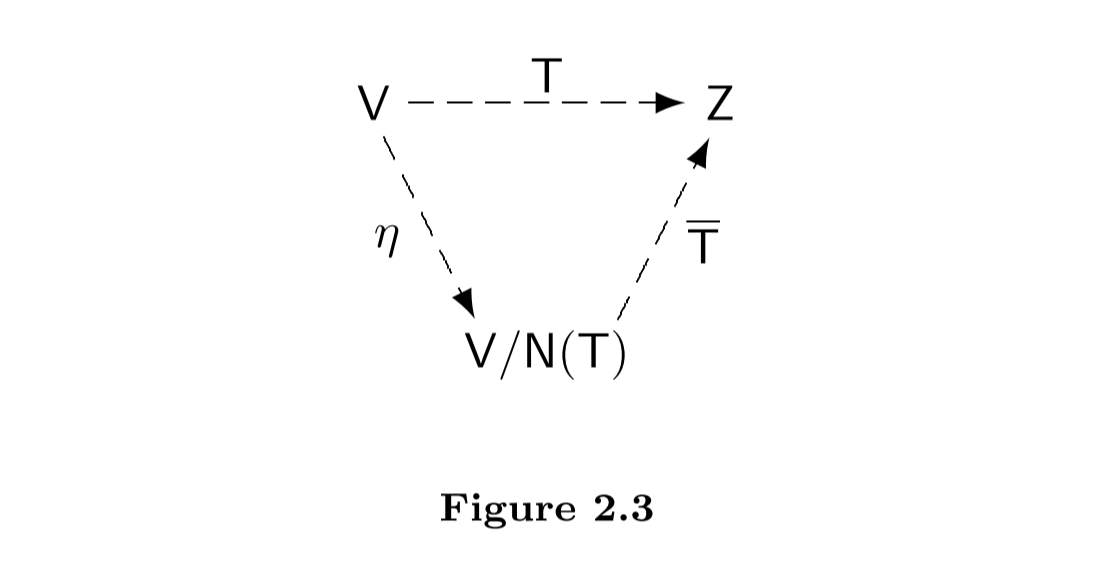
\includegraphics[width=16cm]{images/figure-2-3.png}

\begin{exercise} \label{exercise 2.4.24}
Let \(V\) and \(Z\) be vector spaces and \(\T : V \to Z\) be a linear transformation \emph{that is onto}.
Define the mapping
\[
    \overline{\T} : V / \NULLT \to Z \text{ by } \overline{\T}(v + \NULLT) = \T(v)
\]
for any coset \(v + \NULLT\) in \(V / \NULLT\).
\begin{enumerate}
\item Prove that \(\overline{\T}\) is \emph{well-defined};
    that is, prove that if \(v + \NULLT = v' + \NULLT\), then \(\T(v) = \T(v')\).
\item Prove that \(\overline{\T}\) is linear.
\item Prove that \(\overline{\T}\) is an isomorphism.
\item Prove that the diagram shown in Figure 2.3 \emph{commutes};
    that is, prove that \(\T = \overline{\T} \eta\). (\(\eta\) is defined in \EXEC{2.1.42}.)
\end{enumerate}

Note that we do not say \(V\) and \(Z\) are finite dimensional.
\end{exercise}

\begin{proof} \ 

\begin{enumerate}
\item Suppose \(v + \NULLT = v' + \NULLT\), then by \ATHM{1.10}(b), \(v - v' \in \NULLT\), which implies \(\T(v - v') = 0_{_Z}\), that is, \(\T(v) - \T(v') = 0_{_Z}\), that is, \(\T(v) = \T(v')\).

\item For any \(v_1 + \NULLT\) and \(v_2 + \NULLT\) in \(V/\NULLT\), and any scalar \(c\),
\begin{align*}
    & \overline{\T}\bigg( \big( v_1 + \NULLT \big) + c \big(v_2 + \NULLT \big)  \bigg) \\
    & = \overline{\T}\big( (v_1 + cv_2) + \NULLT) \big) & \text{by def of coset \(+\) and scalar \(\cdot\), see \EXEC{1.3.31}} \\
    & = \T(v_1 + cv_2) & \text{by def of \(\overline{\T}\)} \\
    & = \T(v_1) + c\T(v_2) & \text{since \(\T\) is linear} \\
    & = \overline{\T}(v_1 + \NULLT) + c\overline{\T}(v_2 + \NULLT), & \text{by def of \(\overline{\T}\)}
\end{align*}
hence by \ATHM{2.1}(b), \(\overline{\T}\) is linear.

\item Now we have to show \(\overline{\T}\) is one-to-one and onto.
For one-to-one, suppose \(v + \NULLT \in \NULL(\overline{\T})\), we have to show \(v + \NULLT = \OV + \NULLT\).
Then by definition of \(\overline{\T}\), \(\overline{\T}(v + \NULLT) = \T(v) = 0_{_Z}\), which implies \(v \in \NULLT\).
And of course \(v - \OV \in \NULLT\), so by \ATHM{1.10}(b), \(v + \NULLT = \OV + \NULLT\), as desired.

For onto, suppose arbitrary \(z \in Z\).
\emph{Then since \(\T\) is onto}, we can find \(v \in V\) such that \(\T(v) = z\), and for such \(v\) of course we can find \(v + \NULLT \in V/\NULLT\) such that \(\overline{\T}(v + \NULLT) = \T(v) = z\).
Hence \(\overline{\T}\) is onto.

Hence \(\overline{\T}\) is an isomorphism from \(V/\NULLT\) to \(Z\).

\item It's somewhat ambiguous that the exercise does not mention the corresponding \(W\) of the linear map \(\eta\).
Anyway, we assume \(\eta : V \to V/\NULLT\) by \(\eta(v) = v + \NULLT\).
Then for all \(v \in V\), we have
\begin{align*}
    \overline{\T}\eta(v) & = \overline{\T}(\eta(v)) & \text{by def of composition} \\
                         & = \overline{\T}(v + \NULLT) & \text{by def of \(\eta\)} \\
                         & = \T(v) & \text{by def of \(\overline{\T}\)}
\end{align*}
Hence \(\T = \overline{\T}\eta\).
\end{enumerate}
\end{proof}

\begin{exercise} \label{exercise 2.4.25}
\TODOREF{} \RED{Skip}, this need section 1.7.
\end{exercise}

\begin{proof}
\end{proof}

\begin{additional theorem} \label{athm 2.36}
This is the placeholder theorem for some matrix inversion equations:

\BLUE{(1)} \EXEC{2.4.4}: \((AB)^{-1} = B^{-1} A^{-1}\) when \(A, B\) are invertible (and compatible).

\BLUE{(2)} \EXEC{2.4.5}: \((A^\top)^{-1} = (A^{-1})^\top\) when \(A\) is invertible.
\end{additional theorem}

\begin{additional theorem} \label{athm 2.37}
This is the placeholder theorem for some judgement of zero matrix and invertibility:

\BLUE{(1)} \EXEC{2.4.6}: If \(A\) is invertible and \(AB = O\), then \(B = O\).

\EXEC{2.4.7}:

\BLUE{(2.1)}: If \(A^2 = O\) then \(A\) is not invertible.

\BLUE{(2.2)}: If \(AB = O\) for some \emph{nonzero} \(n \X n\) matrix \(B\), then \(A\) is not invertible.

\BLUE{(3)} \EXEC{2.4.9}: If \(A\) and \(B\) be \(n \X n\) matrices such that \(AB\) is invertible, then both \(A\) and \(B\) are invertible.
\end{additional theorem}

\begin{additional theorem} \label{athm 2.38}
This is the placeholder theorem for \EXEC{2.4.10}:

\BLUE{(1)}: If \(A, B\) are \(n \X n\) squares and \(AB = I_n\), then \(A, B\) are invertible, and \(A = B^{-1}\) and \(B = A^{-1}\).
In fact, we do not need to check \(BA = I_n\), hence a ``one-sided'' inverse is a ``two-sided'' inverse.

\BLUE{(2)}: Analogous result for \LTRAN{}:
Let \(\T : V \to W\) and \(\U : W \to V\) where \(V, W\) have same (finite) dimensions and \(\U\T = \ITRANV\).
Then both \(\U, \T\) are invertible. and we have \((\T)^{-1} = \U\) (hence \(\U^{-1} = \T\)).
\end{additional theorem}

\begin{additional theorem} \label{athm 2.39}
This is the placeholder theorem for \EXEC{2.4.15}:
If \(\T : V \to W\) is a \LTRAN{}, and \(\beta\) is a basis for \(V\), then \(\T\) is an isomorphism (from \(V\) to \(W\)) if and only if \(\T(\beta)\) is a basis for \(W\).
\end{additional theorem}

\begin{additional theorem} \label{athm 2.40}
This is the placeholder theorem for \EXEC{2.4.16}:
Given \(n \X n\) invertible matrix \(B\),
\(\Phi : M_{n \X n}(F) \to M_{n \X n}(F)\) by \(\Phi(A) = B^{-1}AB\) is an isomorphism.
\end{additional theorem}

\begin{additional theorem} \label{athm 2.41}
This is the placeholder theorem for \EXEC{2.4.17}:
Let \(V\) and \(W\) be finite-dimensional vector spaces and \(\T : V \to W\) be an isomorphism.
Let \(V_0\) be a \emph{subspace} of \(V\).
Then

\BLUE{(1)} \(\T(V_0)\) is a subspace of \(W\), and

\BLUE{(2)} \(\dim(V_0) = \dim(\T(V_0))\);
    we say that an isomorphism is \emph{rank-preserving}, since in particular \(\dim(V) = \dim(\T(V))\).
\end{additional theorem}

\begin{additional theorem} \label{athm 2.42}
This is the placeholder theorem for \EXEC{2.4.20}:
Let \(\T: V \to W\) be a linear transformation from an \(n\)-dimensional vector space \(V\) to an \(m\)-dimensional vector space \(W\).
Let \(\beta\) and \(\gamma\) be ordered bases for \(V\) and \(W\), respectively.
Then \(\rankT = \rank(\LMTRAN_A)\) and that \(\nullityT = \nullity(\LMTRAN_A)\), where \(A = [\T]_{\beta}^{\gamma}\).
\end{additional theorem}

\begin{additional theorem} \label{athm 2.43}
This is the placeholder theorem for \EXEC{2.4.21}, which gives an isomorphism \(\Phi_{\beta}^{\gamma} : \mathcal{L}(V, W) \to M_{m \X n}(F)\).
\end{additional theorem}

\begin{additional theorem} \label{athm 2.44}
This is the placeholder theorem for \EXEC{2.4.22}, which gives an isomorphism from \(\POLYNF\) to \(F^{n + 1}\);
And this isomorphism is related to Lagrange polynomials(or \RMK{1.6.6}).
\end{additional theorem}

\begin{additional theorem} \label{athm 2.45}
This is the placeholder theorem for \EXEC{2.4.24}, which gives some other facts about quotient space.
\end{additional theorem}